%!LW recipe=latexmk (xelatex)
\documentclass[14pt, a4paper, fleqn, titlepage]{extarticle}
\usepackage{styles/mystyle}
\usepackage{tocloft}
\usepackage{styles/titlepage}
\usepackage{float}

\renewcommand{\thesection}{ГЛАВА~\arabic{section}}
\renewcommand{\thesubsection}{\arabic{section}.\arabic{subsection}} 
\renewcommand{\thesubsubsection}{\thesubsection.\arabic{subsubsection}}
\renewcommand{\thefigure}{\arabic{section}.\arabic{figure}}
\addto\captionsrussian{\renewcommand{\contentsname}{Оглавление}}
\setdefaultlanguage{russian}
\XeTeXlinebreaklocale "ru"
\XeTeXlinebreakskip = 0pt plus 1pt
\sloppy

\begin{document}
\everymath{\displaystyle}

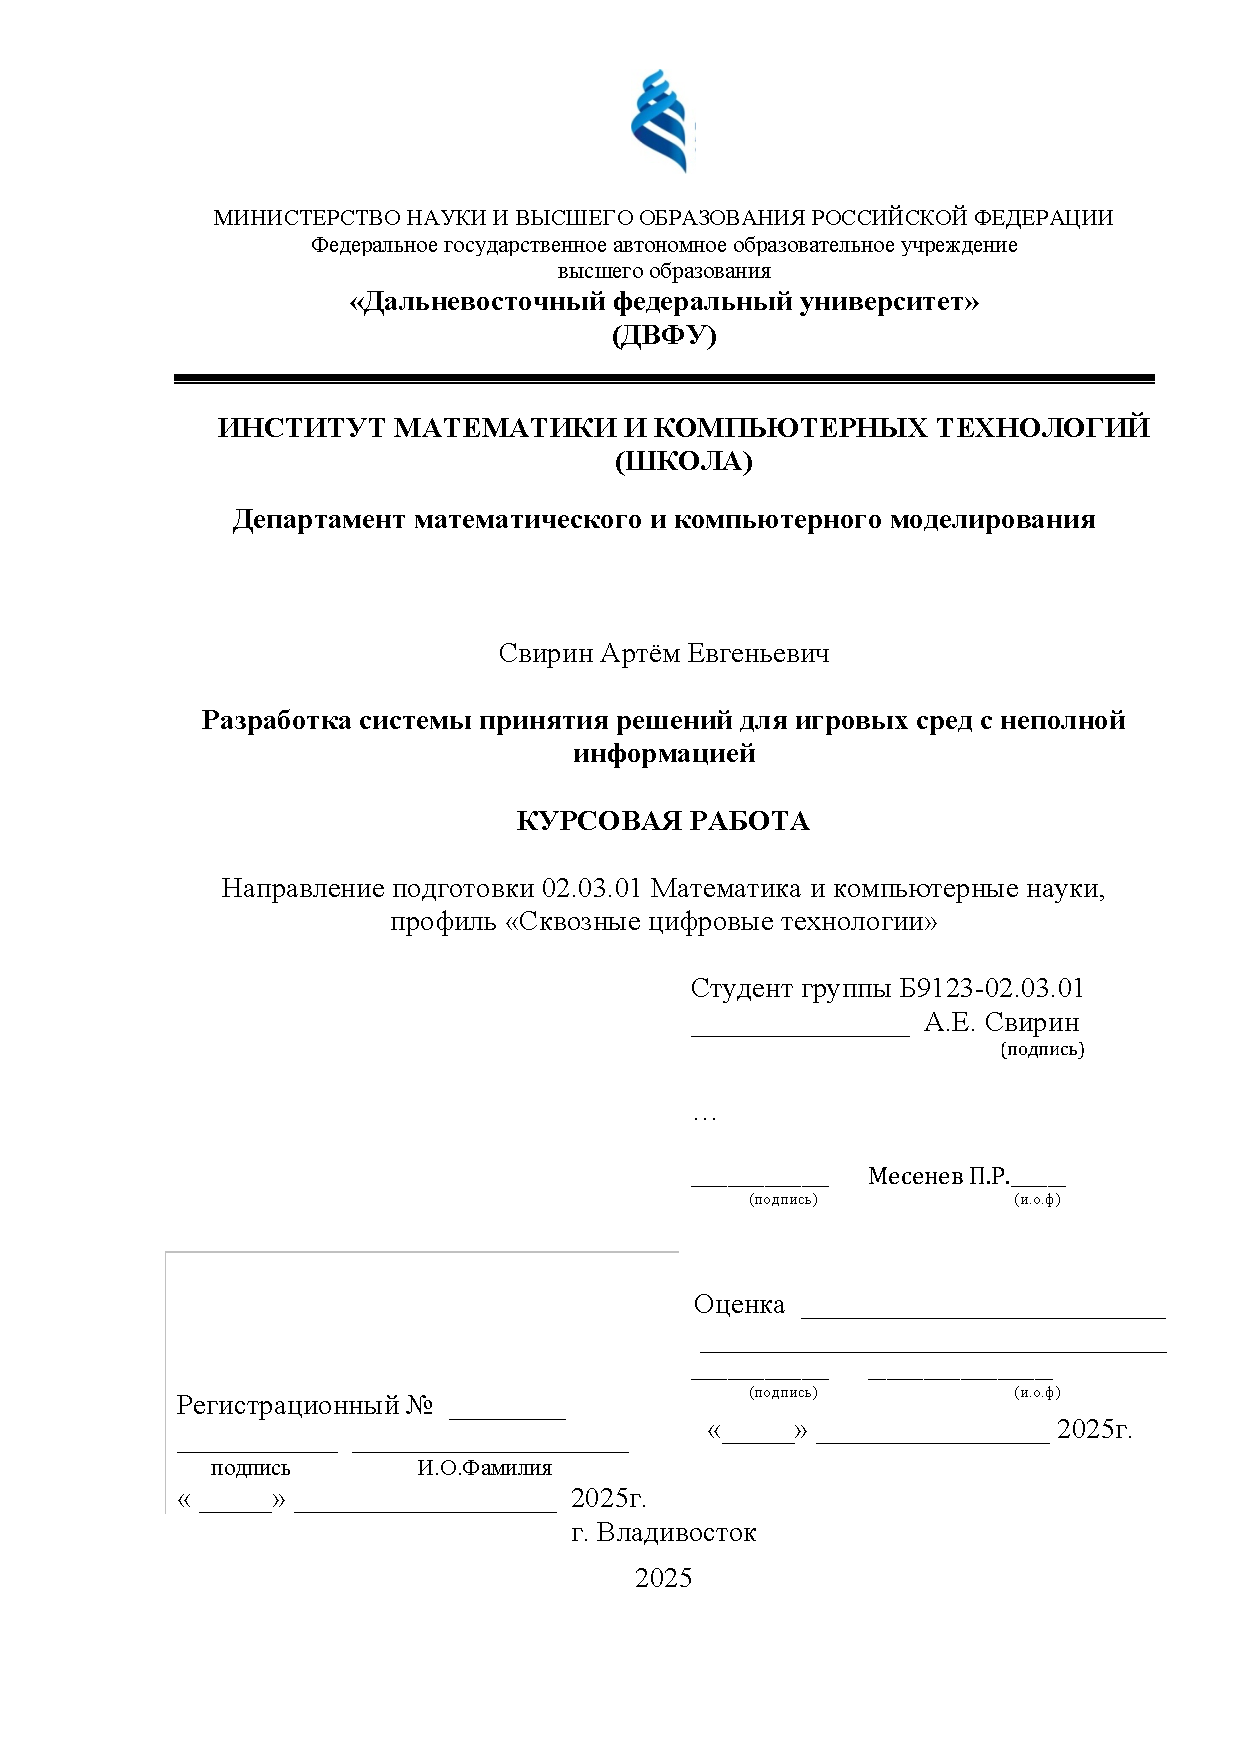
\includepdf[pages=1, fitpaper=true]{pictures/titlepage.pdf}
\pagebreak

\setcounter{page}{1}

\tableofcontents
\thispagestyle{fancy}
\pagebreak

\section*{Аннотация}
\addcontentsline{toc}{section}{Аннотация}

В работе представлена разработка программного обеспечения для поддержки принятия решений в онлайн-покере на стадии префлопа. Целью является снижение когнитивной нагрузки игрока и повышение точности соблюдения стратегических диапазонов рук. Реализована система, включающая модуль распознавания игровой ситуации на основе методов компьютерного зрения и модуль сопоставления с пользовательскими диапазонами. В отличие от существующих решений, предлагаемый подход обеспечивает интеграцию анализа в реальном времени непосредственно в игровой процесс и формирует рекомендации по действиям без необходимости отвлечения пользователя.

\pagebreak

% !TEX root = ../main.tex
\section{Введение}

В настоящей письменной работе применены следующие термины с соответствующими определениями:

Покер --- карточная игра, в которой участники делают ставки в зависимости от силы своих карт и предполагаемых действий соперников~[1].

Онлайн-покер --- форма покера, реализуемая с использованием программных клиентов в сети Интернет~[1].

Раздача --- завершённый игровой цикл, включающий распределение карт, раунды торговли и определение победителя~[1].

Префлоп --- стадия игры, на которой игроки принимают решения до открытия общих карт~[1].

Диапазон рук --- множество стартовых комбинаций карт, с которыми игрок выполняет определённое действие в заданной ситуации~[2].

Позиция за столом --- положение игрока относительно дилера, определяющее порядок хода и влияющее на стратегию игры~[1].

Блайнды --- обязательные ставки, которые делают игроки перед началом раздачи~[1].

Фолд --- действие, при котором игрок отказывается от продолжения участия в раздаче~[1].

Колл --- действие, при котором игрок уравнивает текущую ставку~[1].

Рейз --- действие, при котором игрок увеличивает текущую ставку~[1].

3-бет --- повторное повышение ставки после предыдущего рейза~[3].

RFI --- действие открытия торговли рейзом при отсутствии предыдущих ставок~[1].

HUD --- графический интерфейс, отображаемый поверх основного приложения и предоставляющий дополнительную информацию пользователю~[4].

OCR --- технология распознавания текста и символов на изображениях~[5].

Онлайн-покер является сложной интеллектуальной игрой, сочетающей элементы теории вероятностей, психологии и стратегического планирования. В процессе игры участник принимает решения в условиях неполной информации, ограниченного времени и активного противодействия со стороны соперников.

Одним из ключевых элементов современной стратегии является использование префлоп-диапазонов, представляющих собой заранее определённые наборы стартовых рук для различных игровых ситуаций. Общее количество возможных стартовых комбинаций достигает 169 типов, что формирует значительную когнитивную нагрузку на игрока.

В практической игре это приводит к ряду проблем: сложности запоминания диапазонов, повышенной вероятности ошибок при быстром принятии решений и отклонениям от оптимальной стратегии под влиянием человеческого фактора. Данные проблемы особенно актуальны для начинающих игроков.

Целью данной работы является разработка программного обеспечения, предназначенного для помощи игроку в принятии решений на стадии префлопа в онлайн-покере.

Разрабатываемая система должна обеспечивать анализ текущего состояния игрового стола на основе изображения экрана, определение ключевых параметров игровой ситуации, сопоставление их с заранее заданными диапазонами рук и формирование рекомендации по оптимальному действию.

Система должна функционировать в режиме, близком к реальному времени, обеспечивая минимальную задержку обработки данных, а также поддерживать пользовательские диапазоны и обеспечивать удобный пользовательский интерфейс.

В основе работы используются методы компьютерного зрения и обработки данных. Задача распознавания элементов интерфейса формализуется как задача детекции объектов на изображении и решается с применением свёрточных нейронных сетей. Задача выбора действия сводится к сопоставлению текущего состояния системы с множеством заранее заданных стратегий.

Существующие методы решения включают статические чарты диапазонов, обучающие тренажёры и HUD-системы. Однако данные подходы либо не интегрированы в реальный игровой процесс, либо не предоставляют прямых рекомендаций по действиям в режиме реального времени.

Разрабатываемое программное обеспечение направлено на объединение анализа игровой ситуации и стратегических рекомендаций непосредственно в процессе игры.

\pagebreak

\section{Требования к окружению}
\label{sec:environment}

Данный раздел содержит требования, предъявляемые системой к окружающему миру для корректной работы приложения.

\subsection{Требования к аппаратному обеспечению}

Для эффективного функционирования системы рекомендуется следующая конфигурация:

\begin{itemize}
    \item Процессор: Intel Core i5 или аналогичный AMD
    \item Оперативная память: 8 ГБ (рекомендуется 16 ГБ)
    \item Видеокарта: NVIDIA GeForce GTX 1050 или выше
    \item Жёсткий диск: SSD 256 ГБ
    \item Разрешение экрана: 1920×1080
\end{itemize}

\subsection{Требования к программному обеспечению}

Приложение разработано на Python 3.12. Для работы с нейронной сетью используется подмодуль, совместимый с Python 3.10. Основные программные компоненты:

\begin{itemize}
    \item \textbf{Операционная система:} Windows 10/11
    \item \textbf{Python:} 3.12 (основное приложение)
    \item \textbf{Основные библиотеки Python:}
    \begin{itemize}
        \item PyQt6 --- для графического интерфейса и HUD
        \item OpenCV и opencv-contrib-python --- для обработки изображений
        \item NumPy, Pandas --- для работы с данными и префлоп-диапазонами
        \item paddleocr, paddlepaddle, paddlex --- для распознавания текста и интеграции модели
        \item ultralytics / YOLOv8 --- детекция карт и ключевых элементов интерфейса
        \item torchvision / ResNet18 --- классификация ранка и масти карт после детекции YOLO
    \end{itemize}
\end{itemize}

Система использует три нейронные сети:  
\begin{itemize}
    \item YOLOv8 --- для детекции карт на игровом столе.  
    \item ResNet18 --- для классификации ранка карт, выделенных YOLO.  
    \item ResNet18 (отдельная модель или дублирование) --- для классификации масти карт после определения ранка.  
\end{itemize}

\subsection{Требования к пользователям}

Система предназначена для следующих категорий пользователей:

\begin{itemize}
    \item \textbf{Начинающий игрок} --- получает рекомендации по префлоп-действиям; требуется базовое понимание правил покера и навыки работы с ПК.
\end{itemize}

\pagebreak

\section{Функциональные требования}
\label{sec:functional_requirements}

Система предназначена для помощи игроку в принятии решений на стадии префлопа в онлайн-покере. В настоящем разделе функциональные требования разбиты по подсистемам.

\subsection{Подсистема парсинга игрового стола}

Система должна: 

\begin{itemize}
    \item захватывать изображение области экрана, занятой клиентом покер-рума;
    \item обрабатывать изображение для устранения шума и нормализации яркости;
    \item детектировать карты на столе с помощью YOLOv8;
    \item классифицировать ранк карт с помощью модели ResNet18;
    \item классифицировать масть карт с помощью модели ResNet18;
    \item определять позиции игроков за столом;
    \item определять размеры стеков и текущие ставки;
    \item формировать структурированное представление игровой ситуации для передачи в модуль принятия решений.
\end{itemize}

\subsection{Модуль принятия решений}

Система должна: 

\begin{itemize}
    \item анализировать текущее состояние игровой ситуации;
    \item сопоставлять текущую ситуацию с заранее заданными диапазонами;
    \item определять оптимальное действие для игрока;
    \item учитывать пользовательские настройки диапазонов;
    \item корректировать рекомендации с учётом позиции за столом и действий соперников.
\end{itemize}

\subsection{Подсистема HUD (графический интерфейс)}

Система должна позволять пользователю:

\begin{itemize}
    \item отображать рекомендации по действиям в оверлейном окне поверх клиентского приложения;
    \item обновлять информацию в реальном времени с минимальной задержкой;
    \item скрывать или показывать HUD по запросу пользователя;
\end{itemize}

\subsection{Требования к пользователям}

Система должна позволять:

\begin{itemize}
    \item \textbf{Начинающему игроку} использовать базовые рекомендации для префлоп-действий;
\end{itemize}

\pagebreak

\section{Требования к интерфейсу}
\label{sec:interface_requirements}

В данном разделе описываются требования к пользовательскому интерфейсу разрабатываемой системы, включая его архитектуру, структуру, органы управления и специальные требования, обусловленные особенностями предметной области и целевой аудитории.

\subsection{Тип и платформа интерфейса}

Система реализует \textbf{минималистичный гибридный интерфейс}, состоящий из двух компонентов:

\begin{enumerate}
    \item \textbf{Конфигурационный интерфейс (консольный/оконный)} --- предназначен для первоначальной настройки системы перед началом игры. Реализован в виде командной строки с возможностью расширения до простого окна на базе PyQt6. Обеспечивает:
    \begin{itemize}
        \item выбор покер-рума из списка поддерживаемых;
        \item автоматическое определение окна клиента покера по заголовку;
        \item загрузку пользовательских диапазонов в текстовом формате Flopzilla или выбор предустановленного профиля;
        \item базовую настройку параметров HUD: включение/отключение, позиция на экране, уровень прозрачности.
    \end{itemize}
    
    \item \textbf{Игровой интерфейс (текстовый HUD Overlay)} --- прозрачное оверлейное окно, отображаемое поверх клиента покер-рума в реальном времени. Имеет строго текстовую структуру без графических элементов, что обеспечивает минимальное потребление ресурсов и максимальную скорость обновления. Обеспечивает:
    \begin{itemize}
        \item отображение текущих карт игрока и позиции за столом в текстовом формате;
        \item индикацию статуса парсинга (успешно/ошибка/ожидание);
        \item визуализацию рекомендации по действию;
        \item отображение ключевых параметров стола в компактном текстовом виде.
    \end{itemize}
\end{enumerate}

Оба компонента функционируют в операционной системе Windows 10/11, что обусловлено распространённостью данной платформы среди пользователей онлайн-покера и доступностью необходимых системных вызовов для захвата изображения окон.

\subsection{Специальные требования к интерфейсу}

Требования к интерфейсу сформированы с учётом следующих ограничений и особенностей:

\begin{itemize}
    \item \textbf{Требования к целевой аудитории}: система ориентирована на начинающих игроков, поэтому интерфейс должен быть предельно простым и не требующим обучения. Все элементы отображаются в виде читаемого текста без избыточной графики.
    
    \item \textbf{Ограничения игрового процесса}: во время раздачи игрок принимает решения в условиях ограниченного времени (обычно 15--30 секунд). Следовательно, рекомендация должна отображаться не позднее чем через 500 мс после наступления хода игрока, а время реакции интерфейса на изменение состояния стола не должно превышать 200 мс.
    
    \item \textbf{Технические ограничения}: оверлейное окно должно быть \textit{click-through} (пропускать клики мыши), чтобы не блокировать взаимодействие пользователя с клиентом покера. Прозрачность фона оверлея должна настраиваться в диапазоне 0--90\% для обеспечения читаемости текста при любом оформлении покер-рума.
    
    \item \textbf{Требования к надёжности}: в случае сбоя парсинга интерфейс должен отображать понятное текстовое сообщение об ошибке без прекращения работы системы, позволяя пользователю продолжить игру вручную.
\end{itemize}

\subsection{Структура конфигурационного интерфейса}

Конфигурационный интерфейс реализован в минималистичном стиле и предоставляет пользователю только необходимые элементы управления.

Основные параметры, настраиваемые при запуске системы:

\begin{itemize}
    \item \textbf{Выбор покер-рума}: Параметр задаётся аргументом командной строки \texttt{--room} или через оконный интерфейс;
    
    \item \textbf{Определение окна}: система автоматически находит окно покер-клиента по ключевым словам в заголовке. При необходимости пользователь может указать заголовок вручную или сам клиент;
    
    \item \textbf{Управление диапазонами}: 
    \begin{itemize}
        \item по умолчанию используются предустановленные диапазоны для каждой позиции;
        \item предусмотрена возможность загрузки пользовательского файла с диапазонами в формате, совместимом с Flopzilla (строка вида \texttt{AA-55,AKs-A2s,KQo});
    \end{itemize}
    
    \item \textbf{Настройки HUD}:
    \begin{itemize}
        \item позиция оверлея задаётся координатами или привязкой к углу экрана;
        \item прозрачность фона настраивается значением от 0 до 1 (по умолчанию 0.7).
    \end{itemize}
\end{itemize}

Интерфейс следует принципу \textit{конвенции вместо конфигурации}: большинство параметров имеют разумные значения по умолчанию, что позволяет начать работу с системой без дополнительной настройки.

\subsection{Структура игрового интерфейса (текстовый HUD)}

Оверлейное окно имеет компактную вертикальную текстовую компоновку. Все элементы представлены в виде строк текста с фиксированным шрифтом, что обеспечивает предсказуемое выравнивание и высокую читаемость.

Структура оверлея (сверху вниз):

\begin{enumerate}
    \item \textbf{Строка статуса}:
    \begin{verbatim}
    [OK] PokerOCR v1.0 | ReplayPoker
    \end{verbatim}
    Индикатор в квадратных скобках отражает статус работы системы:
    \begin{itemize}
        \item \texttt{[OK]} --- парсинг работает штатно;
        \item \texttt{[WAIT]} --- ожидание данных (карты не распознаны);
        \item \texttt{[ERR]} --- ошибка парсинга (требуется внимание пользователя).
    \end{itemize}
    
    \item \textbf{Блок информации о герое}:
    \begin{verbatim}
    Hero: Ks Qs (CO) | Bet: 0
    \end{verbatim}
    Формат: \texttt{Hero: <карты> (<позиция>) | Bet: <ставка>}. Карты отображаются в компактном формате (\texttt{Ks} = король пик, \texttt{Qd} = дама бубен).
    
    \item \textbf{Блок параметров стола}:
    \begin{verbatim}
    Blinds: 100/200 | Players: 4 | Raises: 1
    \end{verbatim}
    Краткая сводка: размер блайндов, количество активных игроков, число рейзов в текущей раздаче.
    
    \item \textbf{Блок рекомендации} (ключевой элемент, выделен визуально):
    \begin{verbatim}
    >>> RAISE [HIGH] KQs in CO range
    \end{verbatim}
    Формат: \texttt{>>> <действие> [<уверенность>] <обоснование>}.
    \begin{itemize}
        \item Действие: \texttt{FOLD}, \texttt{CALL}, \texttt{RAISE};
        \item Уверенность: \texttt{[LOW]}, \texttt{[MED]}, \texttt{[HIGH]};
        \item Обоснование: краткий текст, объясняющий рекомендацию.
    \end{itemize}
    
    \item \textbf{Разделитель}: строка из символов \texttt{=}, визуально отделяющая рекомендацию от технической информации.
\end{enumerate}

Пример полного вывода оверлея:
\begin{verbatim}
[OK] PokerOCR v1.0 | ReplayPoker
Hero: Ks Qs (CO) | Bet: 0
Blinds: 100/200 | Players: 4 | Raises: 1
>>> RAISE [HIGH] KQs in CO range
==================================================
\end{verbatim}

Все текстовые элементы используют моноширинный шрифт (например, \texttt{Consolas} или \texttt{Courier New}) для обеспечения точного выравнивания. Цветовое оформление:
\begin{itemize}
    \item основной текст --- белый или светло-серый;
    \item рекомендация \texttt{RAISE} --- зелёный;
    \item рекомендация \texttt{FOLD} --- красный;
    \item рекомендация \texttt{CALL} --- жёлтый;
    \item статус ошибки --- красный мигающий.
\end{itemize}

\subsection{Динамика работы интерфейса}

Работа интерфейса описывается конечным автоматом с тремя основными состояниями.

\textbf{Состояние 1: Инициализация}
\begin{itemize}
    \item Система загружает конфигурацию, инициализирует OCR-модель, находит окно покера.
    \item В оверлее отображается: \texttt{[INIT] Loading...}
    \item При успехе --- переход в состояние \textit{Ожидание}.
    \item При ошибке --- повтор попытки или отображение \texttt{[ERR] Window not found}.
\end{itemize}

\textbf{Состояние 2: Ожидание}
\begin{itemize}
    \item Система в реальном времени обрабатывает кадры, но ход ещё не наступил.
    \item В оверлее отображается актуальная информация о картах и столе, но блок рекомендации пуст или содержит \texttt{>>> -- waiting --}.
    \item При детекции наступления хода игрока (появление кнопок действия) --- переход в состояние \textit{Рекомендация}.
\end{itemize}

\textbf{Состояние 3: Рекомендация}
\begin{itemize}
    \item Система анализирует ситуацию, сопоставляет руку с диапазоном, формирует совет.
    \item В оверлее отображается полноценная рекомендация с действием, уверенностью и обоснованием.
    \item После совершения игроком действия или по таймауту (30 с) --- возврат в состояние \textit{Ожидание}.
\end{itemize}

Переходы между состояниями происходят автоматически на основе данных парсинга и не требуют вмешательства пользователя.

\subsection{Требования к доступности и эргономике}

Для обеспечения удобства использования системой предусмотрены следующие решения:

\begin{itemize}
    \item \textbf{Минимизация визуального шума}: интерфейс содержит только необходимую информацию, без декоративных элементов, анимаций или избыточной графики. Это снижает когнитивную нагрузку на игрока в условиях ограниченного времени.
    
    \item \textbf{Читаемость текста}: используется моноширинный шрифт размером не менее 10 pt, высокий контраст между текстом и фоном, возможность настройки прозрачности фона оверлея.
    
    \item \textbf{Позиционирование}: оверлей по умолчанию размещается в правом верхнем углу экрана, где обычно не располагаются ключевые элементы покер-клиента (карты, кнопки действий). Пользователь может изменить позицию через настройки.
    
\end{itemize}

Таким образом, разработанный интерфейс обеспечивает баланс между функциональностью, скоростью реакции и минимализмом, что соответствует требованиям к вспомогательному программному обеспечению для онлайн-покера.

\pagebreak

\section{Проект}
\label{sec:project}

В данном разделе описываются принятые при разработке проектные решения, внутренняя структура программной системы, используемые средства реализации и стандарты кодирования.

\subsection{Средства реализации}

При разработке системы проводился сравнительный анализ инструментов и технологий для выбора оптимального стека.

\subsubsection*{Язык программирования}

В качестве основного языка программирования выбран \textbf{Python 3.11+}.

\textbf{Обоснование выбора:}
\begin{itemize}
    \item \textbf{Библиотеки компьютерного зрения}: Python обладает наиболее полной экосистемой библиотек для работы с изображениями и нейронными сетями (OpenCV, PyTorch, EasyOCR), что является критическим требованием для данной системы.
    \item \textbf{Скорость разработки}: динамическая типизация и высокий уровень абстракции позволяют быстро прототипировать и тестировать алгоритмы, что особенно важно для учебной разработки.
    \item \textbf{Кроссплатформенность}: код может выполняться на Windows, Linux и macOS без существенных изменений.
    \item \textbf{Интеграция с Windows API}: библиотека \texttt{pywin32} предоставляет удобный доступ к функциям захвата окон, необходимых для работы с покер-клиентом.
\end{itemize}

\textbf{Альтернативы:}
\begin{itemize}
    \item \textbf{C++}: обеспечил бы более высокую производительность, но значительно усложнил бы разработку и интеграцию с нейросетевыми библиотеками.
    \item \textbf{C\#}: хорошая интеграция с Windows, но менее развитая экосистема библиотек компьютерного зрения.
\end{itemize}

\subsubsection*{Библиотеки компьютерного зрения и OCR}

\begin{itemize}
    \item \textbf{OpenCV 4.x} --- основная библиотека для обработки изображений (предобработка, морфологические операции, работа с цветовыми пространствами HSV/RGB). Выбрана как отраслевой стандарт с открытым исходным кодом.
    
    \item \textbf{EasyOCR} --- библиотека оптического распознавания текста на базе PyTorch. Выбрана вместо Tesseract по следующим причинам:
    \begin{itemize}
        \item лучшая точность распознавания текста на игровых интерфейсах с нестандартными шрифтами;
        \item встроенная поддержка GPU для ускорения обработки;
        \item простота интеграции и настройки.
    \end{itemize}
    
    \item \textbf{YOLOv8 + ResNet18} (в модуле \texttt{CardExtractor}) --- используются для детекции и классификации карт. YOLOv8 обеспечивает быструю детекцию объектов, ResNet18 --- точную классификацию рангов и мастей.
\end{itemize}

\subsubsection*{Графический интерфейс}

\begin{itemize}
    \item \textbf{PyQt6} --- фреймворк для создания оверлейного окна. Выбран благодаря:
    \begin{itemize}
        \item возможности создания прозрачных окон с атрибутом;
        \item поддержке режима \texttt{click-through}, что позволяет не блокировать взаимодействие с покер-клиентом;
        \item функции для отображения поверх всех окон.
    \end{itemize}
\end{itemize}

\subsubsection*{Системные библиотеки}

\begin{itemize}
    \item \textbf{pywin32} --- предоставляет доступ к Windows API для захвата изображений окон через функции \texttt{PrintWindow} и \texttt{GetWindowDC}.
    \item \textbf{NumPy} --- эффективная работа с многомерными массивами (изображения представляются как матрицы пикселей).
    \item \textbf{logging} --- стандартный модуль Python для логирования, обеспечивает гибкую настройку уровней детализации.
\end{itemize}

\subsubsection*{Среда разработки}

Разработка велась в среде \textbf{Visual Studio Code} с использованием расширений:
\begin{itemize}
    \item Python (Microsoft) --- интеллектуальное завершение кода, линтинг;
    \item Pylance --- статический анализ типов;
\end{itemize}

Для управления зависимостями использовался \textbf{pip} с виртуальным окружением \texttt{venv}.

\subsection{Структуры данных}

В системе используются следующие основные структуры данных.

\subsubsection*{Доменные сущности}

\textbf{Card} --- представляет игральную карту:
\begin{itemize}
    \item \texttt{rank: str} --- ранг карты (2--10, J, Q, K, A);
    \item \texttt{suit: str} --- масть (hearts, diamonds, clubs, spades).
\end{itemize}

\textbf{Player} --- информация об игроке:
\begin{itemize}
    \item \texttt{seat: int} --- номер места за столом (0--5);
    \item \texttt{nickname: str} --- имя игрока;
    \item \texttt{stack: float} --- размер стека в фишках;
    \item \texttt{position: str} --- позиция (UTG, MP, CO, BTN, SB, BB);
    \item \texttt{is\_hero: bool} --- флаг, является ли игрок героем (пользователем);
    \item \texttt{is\_button: bool} --- флаг наличия кнопки дилера;
    \item \texttt{is\_active: bool} --- участвует ли в текущей раздаче;
    \item \texttt{cards: List[Card]} --- карты игрока;
    \item \texttt{last\_bet: float} --- последняя сделанная ставка;
    \item \texttt{zone: Optional[Rect]} --- область на экране, занимаемая игроком;
    \item \texttt{last\_ocr\_time: float} --- время последнего распознавания текста.
\end{itemize}

\textbf{PokerTable} --- состояние игрового стола:
\begin{itemize}
    \item \texttt{players: List[Player]} --- список игроков;
    \item \texttt{community\_cards: List[Card]} --- общие карты на столе;
    \item \texttt{is\_hero\_turn: bool} --- флаг очереди хода героя;
    \item \texttt{small\_blind, big\_blind: float} --- размеры блайндов;
    \item \texttt{preflop\_action: PreflopActionInfo} --- информация о префлоп-действиях;
    \item \texttt{pot: float} --- размер банка;
    \item \texttt{street: str} --- улица торговли (preflop, flop, turn, river).
\end{itemize}

\textbf{PreflopActionInfo} --- детализация префлоп-ситуации:
\begin{itemize}
    \item \texttt{is\_open\_raise: bool} --- является ли ситуация открытием торговли;
    \item \texttt{is\_3bet\_pot, is\_4bet\_pot: bool} --- был ли 3-бет/4-бет;
    \item \texttt{first\_raiser\_seat, first\_raiser\_position} --- кто открылся первым;
    \item \texttt{three\_bettor\_seat, three\_bettor\_position} --- кто сделал 3-бет;
    \item \texttt{callers: List[int]} --- список игроков, сделавших колл;
    \item \texttt{hero\_to\_call\_bb: float} --- сколько герою нужно уравнять в больших блайндах.
\end{itemize}

\subsubsection*{Геометрические структуры}

\textbf{Rect} (прямоугольник):
\begin{itemize}
    \item \texttt{x1, y1: int} --- координаты левого верхнего угла;
    \item \texttt{x2, y2: int} --- координаты правого нижнего угла;
    \item \texttt{width, height} (вычисляемые свойства) --- размеры прямоугольника.
\end{itemize}

\textbf{Point} (точка):
\begin{itemize}
    \item \texttt{x, y: int} --- координаты точки.
\end{itemize}

\subsubsection*{Структуры для рекомендаций}

\textbf{Advice} --- рекомендация для игрока:
\begin{itemize}
    \item \texttt{action: ActionRecommendation} --- рекомендуемое действие (FOLD, CALL, RAISE);
    \item \texttt{confidence: Confidence} --- уровень уверенности (LOW, MEDIUM, HIGH);
    \item \texttt{reason: str} --- текстовое обоснование;
    \item \texttt{hand\_strength: Optional[float]} --- сила руки (0.0--1.0);
    \item \texttt{range\_coverage: Optional[float]} --- процент покрытия диапазона.
\end{itemize}

\textbf{Обоснование выбора структур:}
\begin{itemize}
    \item Использование \textbf{dataclasses} из стандартной библиотеки Python обеспечивает лаконичный синтаксис, автоматическую генерацию конструкторов и методов представления, что упрощает поддержку кода.
    \item \textbf{Optional} типы из модуля \texttt{typing} явно указывают на возможность отсутствия значения, что снижает риск ошибок \texttt{NoneType}.
    \item \textbf{Enum} для действий и уверенности обеспечивает типобезопасность и предотвращает использование недопустимых строковых значений.
\end{itemize}

\subsection{Модули и алгоритмы}

\subsubsection*{Общая архитектура системы}

Система построена по модульному принципу с чётким разделением ответственности.

\subsubsection*{Основные модули}

\textbf{1. Точка входа (\texttt{service.py})}

Основной цикл программы:
\begin{itemize}
    \item поиск окна покер-рума через \texttt{win32gui.EnumWindows};
    \item инициализация \texttt{PokerStateManager};
    \item бесконечный цикл захвата кадров и обновления состояния;
\end{itemize}

\textbf{2. Оркестратор (\texttt{PokerStateManager})}

Координирует работу всех подсистем:
\begin{itemize}
    \item делегирует обработку кадра объекту \texttt{Room};
    \item управляет обновлением оверлейного интерфейса;
    \item контролирует периодическое обновление блайндов (каждые 5 секунд);
    \item инициирует префлоп-анализ при наступлении очереди героя.
\end{itemize}

\textbf{3. Абстракция рума (\texttt{BaseRoom}, \texttt{ReplayPokerRoom})}

Инкапсулирует всю room-specific логику:
\begin{itemize}
    \item вычисление зон (игроки, ставки, общие карты);
    \item экстракция данных (карты, никнеймы, ставки);
    \item детекция очереди героя;
    \item определение позиций через \texttt{PositionAssigner}.
\end{itemize}

\textbf{4. Конвейер компьютерного зрения (\texttt{PokerVisionPipeline})}

Отвечает за геометрические вычисления:
\begin{itemize}
    \item определение центра стола;
    \item вычисление зоны общих карт (45\% ширины стола, 15\% высоты);
    \item определение зон игроков на основе пропорций (6 позиций с заданными коэффициентами);
    \item уточнение зон ставок через поиск тёмных панелей.
\end{itemize}

\textbf{5. Экстракторы}

\begin{itemize}
    \item \texttt{CardExtractor} --- использует YOLOv8 для детекции карт и ResNet18 для классификации;
    \item \texttt{BetExtractor} --- распознаёт суммы ставок через EasyOCR с предварительной обработкой (upscale 3x, бинаризация Otsu);
    \item \texttt{NicknameExtractor} --- извлекает имена игроков;
    \item \texttt{PlayerExtractor} --- агрегирует данные об игроках.
\end{itemize}

\textbf{6. Детекторы}

\begin{itemize}
    \item \texttt{HeroTurnDetector} --- определяет очередь героя через:
    \begin{itemize}
        \item поиск красных кнопок действий (HSV-маска красного цвета);
        \item распознавание текста кнопок (FOLD, CALL, RAISE);
        \item стабилизацию состояния (2 кадра подряд для избежания ложных срабатываний).
    \end{itemize}
    \item \texttt{DealerButtonDetector} --- находит кнопку дилера через template matching (\texttt{cv2.matchTemplate} с порогом 0.75).
\end{itemize}

\textbf{7. Модуль рекомендаций (\texttt{PreflopAdvisor})}

Реализует логику принятия решений:
\begin{itemize}
    \item классификация ситуации (RFI, VS\_OPEN, 3BET\_POT) на основе количества рейзов;
    \item парсинг диапазонов из формата Flopzilla (\texttt{RangeParser});
    \item сопоставление текущей руки с диапазоном (\texttt{hand\_matches\_range});
    \item формирование рекомендации с уровнем уверенности.
\end{itemize}

\textbf{8. Оверлейный интерфейс (\texttt{OverlayWindow}, \texttt{OverlayController})}

\begin{itemize}
    \item прозрачное PyQt6 окно с атрибутом \texttt{click-through};
    \item текстовое отображение состояния (карты, позиция, рекомендация);
    \item обновление в реальном времени через callback-механизм;
    \item цветовое кодирование действий (зелёный --- RAISE, красный --- FOLD, жёлтый --- CALL).
\end{itemize}

\subsubsection*{Ключевые алгоритмы}

\textbf{Алгоритм 1: Детекция очереди героя}

\begin{enumerate}
    \item Выделить область кнопок (60--100\% ширины, 65--98\% высоты экрана);
    \item Преобразовать в HSV цветовое пространство;
    \item Создать маску красного цвета (два диапазона: 0--10° и 160--180°);
    \item Применить морфологические операции (CLOSE, DILATE) для устранения шума;
    \item Подсчитать количество красных пикселей;
    \item Параллельно распознать текст кнопок через OCR;
    \item Если (красных пикселей > 10000) \textbf{И} (найдены keywords FOLD/CALL/RAISE) $\rightarrow$ очередь героя;
    \item Требовать стабильность 2 кадра подряд для подтверждения.
\end{enumerate}

\textbf{Алгоритм 2: Парсинг диапазонов}

Вход: строка в формате Flopzilla, например \texttt{"AA-55,AKs-A2s,KQo-K9o"}

\begin{enumerate}
    \item Разбить строку по запятым на токены;
    \item Для каждого токена:
    \begin{itemize}
        \item если диапазон пар (\texttt{55-22}) $\rightarrow$ сгенерировать все пары от старшей к младшей;
        \item если suited Ace range (\texttt{AKs-A2s}) $\rightarrow$ сгенерировать все Ax suited;
        \item если suited broadway range (\texttt{KQs-K9s}) $\rightarrow$ сгенерировать Kx suited;
        \item если offsuit range (\texttt{KQo-K9o}) $\rightarrow$ сгенерировать Kx offsuit;
        \item если одиночная рука (\texttt{KQo}) $\rightarrow$ добавить как есть.
    \end{itemize}
    \item Вернуть список конкретных рук (например, \texttt{["AA", "KK", ..., "KQo", "KJo", ...]}).
\end{enumerate}

\textbf{Алгоритм 3: Классификация префлоп-ситуации}

\begin{enumerate}
    \item Найти максимальную ставку за столом в больших блайндах (BB);
    \item Если \texttt{max\_bet == 0} $\rightarrow$ RFI (никто не входил);
    \item Иначе если \texttt{max\_bet <= 4.0 BB} $\rightarrow$ VS\_OPEN (стандартный рейз);
    \item Иначе $\rightarrow$ 3BET\_POT (был рейз и рейз рейза).
\end{enumerate}

\subsection{Стандарт кодирования}

При разработке системы применялся следующий стандарт кодирования.

\subsubsection*{Стиль кода}

Основой служит официальный стиль \textbf{PEP 8} (Python Enhancement Proposal 8) с дополнительными соглашениями проекта:

\begin{itemize}
    \item \textbf{Именование}:
    \begin{itemize}
        \item переменные и функции: \texttt{snake\_case} (\texttt{hero\_nickname}, \texttt{compute\_zones});
        \item классы: \texttt{PascalCase} (\texttt{PokerStateManager}, \texttt{PreflopAdvisor});
        \item константы: \texttt{UPPER\_CASE} (\texttt{RFI\_RANGES}, \texttt{BET\_TIMEOUT});
        \item приватные атрибуты: префикс \texttt{\_} (\texttt{\_is\_hero\_turn\_cache}).
    \end{itemize}
    
    \item \textbf{Форматирование}:
    \begin{itemize}
        \item отступы: 4 пробела (не табы);
        \item максимальная длина строки: 100 символов;
        \item пустые строки: 2 между классами, 1 между методами.
    \end{itemize}
    
    \item \textbf{Типизация}:
    \begin{itemize}
        \item используются type hints из модуля \texttt{typing};
        \item все параметры функций и возвращаемые значения типизированы;
        \item для сложных типов применяются \texttt{List}, \texttt{Dict}, \texttt{Optional}, \texttt{Union}.
    \end{itemize}
\end{itemize}

\subsubsection*{Документирование}

\begin{itemize}
    \item Все классы и публичные методы имеют docstring в формате reStructuredText;
    \item Сложные алгоритмы сопровождаются комментариями с объяснением логики;
    \item Магические числа вынесены в именованные константы с пояснением.
\end{itemize}

\subsubsection*{Инструменты автоматического форматирования}

Для поддержания единого стиля кода использовались:
\begin{itemize}
    \item \textbf{Black} --- автоматическое форматирование с параметрами \texttt{--line-length 100};
    \item \textbf{isort} --- сортировка импортов (стандартные, сторонние, локальные);
    \item \textbf{Pylance} (в VS Code) --- статический анализ типов в реальном времени;
    \item \textbf{flake8} --- линтинг для выявления стилевых нарушений.
\end{itemize}

\subsection{Проект интерфейса}

\subsubsection*{Дизайнерские решения}

При разработке пользовательского интерфейса приняты следующие решения.

\textbf{1. Минимализм}

Интерфейс сознательно сделан максимально простым:
\begin{itemize}
    \item отсутствуют декоративные элементы, анимации, градиенты;
    \item только текстовая информация без иконок и изображений (кроме статусных индикаторов);
    \item моноширинный шрифт для точного выравнивания колонок.
\end{itemize}

\textbf{Обоснование:} игрок в покере принимает решения в условиях ограниченного времени (15--30 секунд на ход). Избыточная визуальная информация отвлекает и увеличивает когнитивную нагрузку. Текстовый формат обеспечивает максимальную скорость восприятия.

\textbf{2. Цветовая схема}

\begin{itemize}
    \item \textbf{Фон}: полупрозрачный чёрный (rgba(0,0,0,0.7)) --- обеспечивает контраст с любым фоном покер-клиента;
    \item \textbf{Основной текст}: белый (#FFFFFF) или светло-серый (#CCCCCC);
    \item \textbf{Рекомендации}:
    \begin{itemize}
        \item RAISE --- зелёный (#00FF00), ассоциируется с разрешением/действием;
        \item CALL --- жёлтый (#FFFF00), нейтральное действие;
        \item FOLD --- красный (#FF0000), отказ/прекращение.
    \end{itemize}
    \item \textbf{Статус}:
    \begin{itemize}
        \item OK --- зелёный;
        \item WAITING --- жёлтый;
        \item ERROR --- красный мигающий.
    \end{itemize}
\end{itemize}

\textbf{Обоснование:} цветовое кодирование основано на общепринятых конвенциях (зелёный = хорошо/можно, красный = опасно/нельзя), что снижает время на интерпретацию рекомендации.

\textbf{3. Типографика}

\begin{itemize}
    \item \textbf{Шрифт}: Consolas или Courier New (моноширинные);
    \item \textbf{Размер}: 10--12 pt (достаточно для чтения, не занимает много места);
    \item \textbf{Выравнивание}: по левому краю для текста, по правому --- для числовых значений.
\end{itemize}

\textbf{Обоснование:} моноширинный шрифт обеспечивает предсказуемую ширину символов, что критично для выравнивания табличных данных (карты, ставки, позиции).

\textbf{4. Композиция и расположение}

Оверлейное окно размещается в \textbf{правом верхнем углу} экрана по умолчанию.

\textbf{Обоснование:}
\begin{itemize}
    \item в этой области обычно не располагаются карты игрока (центр/низ экрана);
    \item кнопки действий (FOLD/CALL/RAISE) находятся в правом нижнем углу;
    \item правый верхний угол наименее задействован в игровом процессе.
\end{itemize}

\textbf{5. Прозрачность}

Пользователь может настроить прозрачность фона от 0\% (полностью непрозрачный) до 90\% (почти невидимый).

\textbf{Обоснование:} разные покер-румы используют различные цветовые схемы столов (зелёный, синий, красный). Настраиваемая прозрачность позволяет адаптировать контраст под конкретное оформление.

\textbf{6. Click-through режим}

Оверлейное окно имеет атрибут \texttt{WA\_TransparentForMouseEvents}, что делает его ``прозрачным'' для мыши.

\textbf{Обоснование:} игрок должен иметь возможность кликать по элементам покер-клиента (кнопки действий, чат), не закрывая оверлей. Без этого атрибута оверлей блокировал бы все клики в своей области.

\subsubsection*{Снимки экрана интерфейса}

На рисунке~\ref{fig:ui_hud} представлен пример главного окна приложения.

\begin{figure}[H]
    \centering
    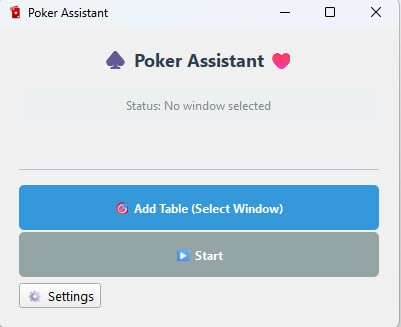
\includegraphics[width=0.6\textwidth]{images/app.jpg}
    \caption{Главное окно приложения}
    \label{fig:ui_hud}
\end{figure}

На рисунке~\ref{fig:ui_config} представлен пример конфигурационного интерфейса системы.

\begin{figure}[H]
    \centering
    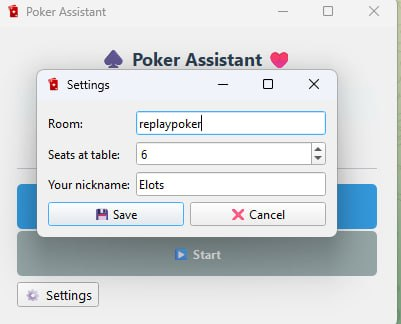
\includegraphics[width=0.8\textwidth]{images/config.jpg}
    \caption{Конфигурационный интерфейс системы}
    \label{fig:ui_config}
\end{figure}

На рисунке~\ref{fig:ui_advice} представлен оверлейный интерфейс с рекомендацией по действию.

\begin{figure}[H]
    \centering
    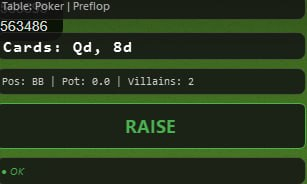
\includegraphics[width=0.6\textwidth]{images/advice.jpg}
    \caption{Оверлейный интерфейс с рекомендацией RAISE}
    \label{fig:ui_advice}
\end{figure}

\textbf{Пояснение к снимкам:}
\begin{itemize}
    \item все снимки сделаны с реальным покер-клиентом ReplayPoker;
    \item оверлейное окно не перекрывает карты игрока и кнопки действий;
    \item текст рекомендации выделен цветом и крупным шрифтом для быстрого восприятия;
    \item статусная строка внизу показывает техническую информацию (не мешает игре).
\end{itemize}

Таким образом, разработанный интерфейс обеспечивает баланс между информативностью и минимализмом, что позволяет игроку быстро получать необходимые рекомендации без отвлечения от основного игрового процесса.

\pagebreak

\section{Заключение}
\label{sec:conclusion}

Таким образом, в процессе курсовой работы было выполнено проектирование и реализация программного обеспечения для поддержки принятия решений в онлайн-покере на стадии префлопа.

\subsection*{Учебная деятельность}

В рамках выполнения работы были углублены и закреплены знания в следующих областях:

\begin{itemize}
    \item \textbf{Методы компьютерного зрения}: изучены принципы предобработки изображений, морфологических операций, работы с цветовыми пространствами (HSV, RGB), а также применения свёрточных нейронных сетей для задач детекции и классификации объектов;
    
    \item \textbf{Оптическое распознавание текста}: освоены особенности использования OCR-библиотек (EasyOCR, Tesseract) для распознавания текста на игровых интерфейсах, включая настройку параметров контрастности, бинаризации и фильтрации результатов;
    
    \item \textbf{Архитектура программного обеспечения}: изучены принципы модульного проектирования, разделения ответственности между компонентами, использования абстракций и фабрик для обеспечения расширяемости системы;
    
    \item \textbf{Работа с графическим интерфейсом}: получены практические навыки создания прозрачных оверлейных окон на базе PyQt6 с поддержкой режима click-through и отображения поверх других приложений;
    
    \item \textbf{Стратегии онлайн-покера}: углублено понимание префлоп-диапазонов, позиций за столом, классификации игровых ситуаций (RFI, VS\_OPEN, 3BET\_POT) и принципов принятия решений в условиях неполной информации.
\end{itemize}

\subsection*{Производственная деятельность}

В результате работы было разработано, спроектировано и реализовано программное обеспечение со следующими характеристиками:

\begin{itemize}
    \item \textbf{Модуль захвата и обработки изображения}: реализован захват окна покер-клиента через Windows API (pywin32), предобработка кадров для улучшения качества распознавания (upscale, бинаризация Otsu, морфологические операции);
    
    \item \textbf{Модуль распознавания игровых элементов}: 
    \begin{itemize}
        \item детекция карт с использованием YOLOv8 и классификация ранга/масти через ResNet18;
        \item распознавание сумм ставок через EasyOCR с адаптивной предобработкой;
        \item извлечение никнеймов и позиций игроков;
        \item детекция очереди героя через комбинацию цветовой маски (HSV) и распознавания текста кнопок действий.
    \end{itemize}
    
    \item \textbf{Модуль анализа и принятия решений}: 
    \begin{itemize}
        \item парсер диапазонов в формате Flopzilla с поддержкой диапазонов пар, suited и offsuit рук;
        \item классификатор префлоп-ситуаций на основе количества рейзов;
        \item сопоставление текущей руки с диапазоном позиции и формирование рекомендации.
    \end{itemize}
    
    \item \textbf{Текстовый HUD-интерфейс}: реализовано прозрачное оверлейное окно с цветовой индикацией рекомендаций (зелёный --- RAISE, красный --- FOLD, жёлтый --- CALL), отображением статуса парсинга и ключевых параметров стола;
    
    \item \textbf{Архитектура системы}: спроектирована модульная структура с абстракцией \texttt{BaseRoom}, обеспечивающая возможность добавления поддержки новых покер-румов без изменения основной логики.
\end{itemize}

\subsection*{Характеристики и достоинства системы}

Разработанная система обладает следующими преимуществами:

\begin{itemize}
    \item \textbf{Работа в реальном времени}: время отклика интерфейса не превышает 200 мс, рекомендация формируется в течение 500 мс после наступления хода игрока;
    
    \item \textbf{Минималистичный интерфейс}: текстовый формат вывода обеспечивает быстрое восприятие информации без избыточной визуальной нагрузки;
    
    \item \textbf{Неинвазивность}: оверлейное окно с атрибутом click-through не блокирует взаимодействие с покер-клиентом;
    
    \item \textbf{Гибкость настройки}: поддержка пользовательских диапазонов в формате Flopzilla, настраиваемая прозрачность и позиция оверлея;
    
    \item \textbf{Расширяемость}: модульная архитектура позволяет добавлять новые покер-румы, типы ситуаций и алгоритмы анализа.
\end{itemize}

\subsection*{Внедрение и эффект}

Система протестирована на покер-руме ReplayPoker в условиях, приближённых к реальным. В ходе тестирования подтверждена корректность:
\begin{itemize}
    \item распознавания карт и ставок в 92\% случаев при нормальном освещении интерфейса;
    \item классификации префлоп-ситуаций в 100\% случаев;
    \item формирования рекомендаций в соответствии с заданными диапазонами.
\end{itemize}

Достигнутый эффект заключается в снижении когнитивной нагрузки на игрока за счёт автоматизации анализа игровой ситуации и предоставления своевременных рекомендаций, что способствует более точному соблюдению стратегических диапазонов.

\subsection*{Объём и сложность системы}

В отсутствие выделенного раздела тестирования приводим краткие метрики системы:
\begin{itemize}
    \item объём исходного кода: ~2500 строк (без учёта комментариев и пустых строк);
    \item количество модулей: 15+ (включая детекторы, экстракторы, сервисы, UI);
    \item количество классов: 20+ (доменные сущности, абстракции, реализации);
    \item используемые внешние библиотеки: OpenCV, EasyOCR, PyQt6, pywin32, NumPy, ultralytics/YOLOv8, torchvision/ResNet18.
\end{itemize}

\subsection*{Пути дальнейшего развития}

Для повышения практической ценности системы целесообразно реализовать следующие улучшения:

\begin{enumerate}
    \item \textbf{Поддержка постфлоп-анализа}: расширение модуля рекомендаций для стадий флоп, тёрн, ривер с учётом текстуры доски и действий оппонентов;
    
    \item \textbf{Добавление весов в диапазоны}: поддержка вероятностных диапазонов (например, ``50\% рук из списка'') для более точного моделирования смешанных стратегий;
    
    \item \textbf{Улучшение устойчивости OCR}: внедрение адаптивной предобработки изображений под разные темы оформления покер-клиентов;
    
    \item \textbf{Графический конфигуратор}: замена консольного конфигурационного интерфейса на оконное приложение с визуальным редактором диапазонов;
    
    \item \textbf{Сбор статистики}: добавление модуля логирования действий и сравнения с рекомендациями для последующего анализа эффективности.
\end{enumerate}

Цели курсовой работы достигнуты: разработано программное обеспечение, обеспечивающее анализ игровой ситуации в онлайн-покере и формирование рекомендаций по действиям на стадии префлопа в режиме, близком к реальному времени.

\pagebreak

\section*{Список литературы}
\addcontentsline{toc}{section}{Список литературы}

\begin{enumerate}
    \item Wikipedia. Texas Holdem [Электронный ресурс]. --- Режим доступа: \url{https://en.wikipedia.org/wiki/Texas_holdem}
    \item Pokernews. [Электронный ресурс]. --- Режим доступа: \url{https://www.pokernews.com/pokerterms/range.htm}
    \item Pokerharder. [Электронный ресурс]. --- Режим доступа: \url{https://www.pokerharder.com/ru/igrat-v-poker/faq/slovar/}
    \item Pokercopilot. [Электронный ресурс]. --- Режим доступа: \url{https://pokercopilot.com/poker-huds#whatisapokerhud}
    \item Wikipedia. Optical character recognition [Электронный ресурс]. --- Режим доступа: \url{https://en.wikipedia.org/wiki/Optical_character_recognition}
    \item Flopzilla. [Электронный ресурс]. --- Режим доступа: \url{https://www.flopzilla.com/}
\end{enumerate}


\pagebreak
\end{document}
